\usepackage[utf8]{inputenc}
\usepackage{graphicx}
\usepackage{listings}
\usepackage{lmodern}
\usepackage[T1]{fontenc}
\usepackage{libertine}
\usepackage{tikz}
\usetikzlibrary{fit,arrows,shapes,backgrounds}
\usepackage{emselip}
\widowpenalty10000
\clubpenalty10000
\brokenpenalty=10000

\usepackage{comment}
\usepackage{float}
\usepackage{microtype}

\usepackage{etoolbox}

% definit un booleen pour inclure ou non les corrections
% par defaut a true
\newtoggle{includematlabcorrection}
\toggletrue{includematlabcorrection}
\newtoggle{includepythoncorrection}
\toggletrue{includepythoncorrection}
\newtoggle{matlabbook}
\toggletrue{matlabbook}
\newtoggle{pythonbook}
\toggletrue{pythonbook}


\newcommand{\inputmatlabcorrection}[1]{\iftoggle{includematlabcorrection}{\input{#1}}{}
}
\newcommand{\inputpythoncorrection}[1]{\iftoggle{includepythoncorrection}{\input{#1}}{}
}
\newcommand{\ifmatlab}[1]{\iftoggle{matlabbook}{#1}{}
}
\newcommand{\ifpython}[1]{\iftoggle{pythonbook}{#1}{}
}

\newcommand{\matlabregistered}{MATLAB\textsuperscript{\textregistered}}
\usepackage{xcolor}

\definecolor{dkgreen}{rgb}{0,0.6,0}
\definecolor{gray}{rgb}{0.5,0.5,0.5}
\definecolor{mauve}{rgb}{0.58,0,0.82}
% colors
\definecolor{darkblue}{rgb}{0,0.1,0.5}
\definecolor{blueemse}{RGB}{0 63 135} % bleu pantone 294 CV / EMSE
\definecolor{ocre}{RGB}{243,102,25} % Define the orange color used for highlighting 
\definecolor{matlabblue}{RGB}{34 85 139} % bleu fenetre matlab

%*******************************************************************************
% couleurs automne
\definecolor{automne_primaire0}{RGB}{ 95, 57, 65}
\definecolor{automne_primaire1}{RGB}{208,193,196}
\definecolor{automne_primaire2}{RGB}{152,112,121}
\definecolor{automne_primaire3}{RGB}{86, 21, 35}
\definecolor{automne_primaire4}{RGB}{64,  0, 14}

\definecolor{automne_complement0}{RGB}{ 66, 89, 54}
\definecolor{automne_complement1}{RGB}{187,196,182}
\definecolor{automne_complement2}{RGB}{119,143,106}
\definecolor{automne_complement3}{RGB}{ 41, 81, 19}
\definecolor{automne_complement4}{RGB}{ 21, 60,  0}

%%% couleurs a utiliser
% code informatique
\colorlet{c_code_numberstyle}{gray} % numerotation de lignes
\colorlet{c_code_keyword}{blueemse} % keyword
\colorlet{c_code_rule}{automne_primaire4} % lignes
\colorlet{c_code_comment}{red} % commentaires
\colorlet{c_code_string}{automne_primaire0} % chaines de caracteres
\colorlet{c_code_colback}{automne_primaire1!10} % fond des fenetres
\colorlet{c_code_colframe}{automne_primaire3} % bordure des fenetres
\colorlet{c_code_icon_fill}{automne_primaire1} % icone: fond
\colorlet{c_code_title}{automne_primaire3} % titre (non utilise)

% fenetres de questions
\colorlet{c_qbox_colback}{automne_primaire1} % fond des fenetres
\colorlet{c_qbox_colframe}{automne_primaire4} % bordure des fenetres
\colorlet{c_qbox_icon_colback}{automne_primaire1!10} % icone: fond
\colorlet{c_qbox_icon_colframe}{automne_primaire3} % icone: bordure

% document
\colorlet{c_title}{automne_complement4}
\colorlet{c_rule}{automne_complement4}
\colorlet{c_page}{automne_complement4}
\colorlet{c_section}{automne_complement4}
\colorlet{c_section_colframe}{automne_complement4} % bordure des fenetres
\colorlet{c_section_colback}{automne_complement1}  % fond des fenetres

% %***************************************************************************
% % % couleur vert orange flashy
% \definecolor{flashy_primaire0}{RGB}{127,234,110 }
% \definecolor{flashy_primaire1}{RGB}{232,255,229}
% \definecolor{flashy_primaire2}{RGB}{172,248,160}
% \definecolor{flashy_primaire3}{RGB}{ 92,207, 74}
% \definecolor{flashy_primaire4}{RGB}{ 58,136, 46}
% 
% \definecolor{flashy_complement0}{RGB}{160, 61, 68}
% \definecolor{flashy_complement1}{RGB}{252,140,148}
% \definecolor{flashy_complement2}{RGB}{228,111,120}
% \definecolor{flashy_complement3}{RGB}{103, 28, 33}
% \definecolor{flashy_complement4}{RGB}{ 43,  7, 10}
% %%% couleurs a utiliser
% % code informatique
% \colorlet{c_code_numberstyle}{gray}
% \colorlet{c_code_keyword}{blueemse}
% \colorlet{c_code_rule}{flashy_primaire4}
% \colorlet{c_code_comment}{red}
% \colorlet{c_code_string}{flashy_primaire0}
% \colorlet{c_code_colback}{flashy_primaire1!10} % fond des fenetres
% \colorlet{c_code_colframe}{flashy_primaire3} % bordure des fenetres
% \colorlet{c_code_icon_fill}{flashy_primaire1}
% \colorlet{c_code_title}{flashy_primaire3}
% 
% % fenetres de questions
% \colorlet{c_qbox_colback}{orange!10} % fond des fenetres
% \colorlet{c_qbox_colframe}{flashy_primaire3} % bordure des fenetres
% \colorlet{c_qbox_icon_colback}{orange!20}
% \colorlet{c_qbox_icon_colframe}{flashy_primaire3}
% 
% % document
% \colorlet{c_title}{flashy_complement3}
% \colorlet{c_rule}{flashy_complement3}
% \colorlet{c_page}{flashy_complement4}
% \colorlet{c_section}{flashy_complement4}
% \colorlet{c_section_colframe}{flashy_complement4} % bordure des fenetres
% \colorlet{c_section_colback}{flashy_complement2}  % fond des fenetres


\usepackage{pdfpages}

\usepackage[%           % Fine in most cases
            pdfpagelabels,hypertexnames=true,
            plainpages=false,
            naturalnames=false,
            pdftitle={Image Processing Tutorials},
				backref=page,
				linktoc=all,
				hidelinks
  			]{hyperref}

\hypersetup{colorlinks,
            linkcolor=c_section,
            anchorcolor=c_section,
            citecolor=c_section}

    
\usepackage{import}
%\subimport{./}{couleurs.tex}
\usepackage{tikz}
\usetikzlibrary{arrows,calc,shapes.geometric,plotmarks}
\usepackage{listings}
\usepackage{tcolorbox}
\tcbuselibrary{listings,skins,breakable}


\usepackage{accsupp}
\newcommand{\noncopynumber}[1]{%
    \BeginAccSupp{method=escape,ActualText={}}%
    #1%
    \EndAccSupp{}%
}


\lstdefinestyle{MatlabStyle} { %
  language=Matlab,                % the language of the code
%  float,
%  floatplacement=htbp,
  basicstyle=\footnotesize,           % the size of the fonts that are used for the code
  numbers=left,                   % where to put the line-numbers
  numberstyle=\tiny\color{c_code_numberstyle}\noncopynumber,  % the style that is used for the line-numbers
  stepnumber=2,                   % the step between two line-numbers. If it's 1, each line 
                                  % will be numbered
  numbersep=5pt,                  % how far the line-numbers are from the code
  %backgroundcolor=\color{white},      % choose the background color. You must add \usepackage{color}
  showspaces=false,               % show spaces adding particular underscores
  showstringspaces=false,         % underline spaces within strings
  showtabs=false,                 % show tabs within strings adding particular underscores
  %frame=single,                   % adds a frame around the code
  %rulecolor=\color{blueemse},        % if not set, the frame-color may be changed on line-breaks within not-black text (e.g. commens (green here))
  tabsize=2,                      % sets default tabsize to 2 spaces
  captionpos=b,                   % sets the caption-position to bottom
  breaklines=true,                % sets automatic line breaking
  breakatwhitespace=false,        % sets if automatic breaks should only happen at whitespace
  title=\lstname,         % show the filename of files included with \lstinputlisting;
                                  % also try caption instead of title
  keywordstyle=\color{c_code_keyword},          % keyword style
  commentstyle=\color{c_code_comment},       % comment style
  stringstyle=\color{c_code_string},         % string literal style
  escapeinside={\%*}{*)},            % if you want to add a comment within your code
  morekeywords={*,...},               % if you want to add more keywords to the set
 % literate=*{-}{-}1  
  columns=flexible
}

\lstdefinestyle{PythonStyle}{ %
  language=Python,                % the language of the code
  basicstyle=\footnotesize,       % the size of the fonts that are used for the code
  numbers=left,                   % where to put the line-numbers
%  float,
%  floatplacement=htbp,
  numberstyle=\tiny\color{c_code_numberstyle},  % the style that is used for the line-numbers
  stepnumber=2,                   % the step between two line-numbers. If it's 1, each line 
                                  % will be numbered
  numbersep=5pt,                  % how far the line-numbers are from the code
  %backgroundcolor=\color{white},  % choose the background color. You must add \usepackage{color}
  showspaces=false,               % show spaces adding particular underscores
  showstringspaces=false,         % underline spaces within strings
  showtabs=false,                 % show tabs within strings adding particular underscores
  %frame=single,                   % adds a frame around the code
  rulecolor=\color{c_code_rule},        % if not set, the frame-color may be changed on line-breaks within not-black text (e.g. commens (green here)) 
  tabsize=2,                      % sets default tabsize to 2 spaces
  captionpos=b,                   % sets the caption-position to bottom
  breaklines=true,                % sets automatic line breaking
  breakatwhitespace=false,        % sets if automatic breaks should only happen at whitespace
  title=\lstname,                   % show the filename of files included with \lstinputlisting;
                                  % also try caption instead of title
  keywordstyle=\color{c_code_keyword},          % keyword style
  commentstyle=\color{c_code_comment},       % comment style
  stringstyle=\color{c_code_string},         % string literal style
 % index=[1][meshgrid],
  escapeinside={\%*}{*)},            % if you want to add a comment within your code
  morekeywords={*,...},               % if you want to add more keywords to the set
  tabsize=3,
  literate=*{-}{-}1
}
% \lstnewenvironment{matlab}
%   {\lstset{language=Matlab,style=MatlabStyle}}
%   {}

\newenvironment{matlab}{%
  \tcblisting{listing only,colback=c_code_colback,colframe=c_code_colframe, enlarge top by=5.5mm,enhanced,breakable,boxrule=1pt,%
     overlay={\node[anchor=west,xshift=10pt,draw=c_code_colframe, line width=2pt, rectangle, rounded corners=2pt,fill=c_code_icon_fill,inner sep=2pt,outer sep=0pt, minimum size=20pt] at (frame.north west) {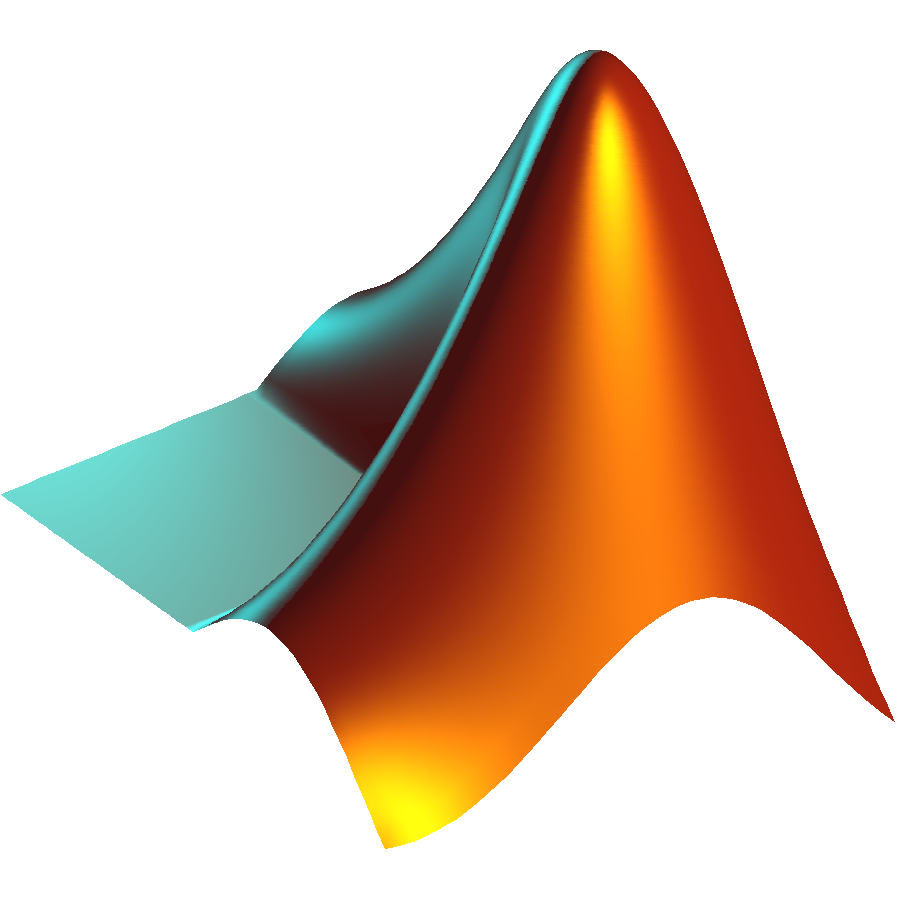
\includegraphics[width=16pt]{matlab-logo.png}};},%
     listing options={basicstyle=\footnotesize\ttfamily,breaklines=true,%
                      postbreak={\mbox{$\hookrightarrow\space$}},%
                      language=Matlab,style=MatlabStyle},%
  }%
 }%
 {\endtcblisting}

\newenvironment{python}{%
  \tcblisting{listing only,colback=c_code_colback,colframe=c_code_colframe, enlarge top by=5.5mm,enhanced,boxrule=1pt,%
     overlay={\node[anchor=west,xshift=10pt,draw=c_code_colframe, line width=2pt, rectangle, rounded corners=2pt,fill=c_code_icon_fill,inner sep=2pt,outer sep=0pt, minimum size=20pt] at (frame.north west) {
\includegraphics[width=16pt]{python-logo.pdf}};},%
     listing options={basicstyle=\footnotesize\ttfamily,breaklines=true,%
                      postbreak={\mbox{$\hookrightarrow\space$}},language=Python,style=PythonStyle},%
  }%
 }%
 {\endtcblisting}
\newenvironment{sh}{%
  \tcblisting{listing only,colback=c_code_colback,colframe=c_code_colframe, enlarge top by=5.5mm,enhanced,boxrule=1pt,%
     overlay={\node[anchor=west,xshift=10pt,draw=c_code_colframe, line width=2pt, rectangle, rounded corners=2pt,fill=c_code_icon_fill,inner sep=2pt,outer sep=0pt, minimum size=20pt] at (frame.north west) {
\includegraphics[width=16pt]{sh-logo.pdf}};},%
     listing options={basicstyle=\footnotesize\ttfamily,breaklines=true,%
                      postbreak={\mbox{$\hookrightarrow\space$}},language=sh,style=PythonStyle},%
  }%
 }%
 {\endtcblisting}


\newcommand{\triangcirc}{\tikz{
\node[circle,white,draw,inner sep=3pt] (c) {};
\node[isosceles triangle,
      white,
      fill,
      rotate=-90,
      anchor=apex,
      isosceles triangle apex angle=60,
      inner sep=1.5pt] (t) at ([yshift=0.5pt]c.south) {};}}
% 
% \makeatletter
% \renewcommand*\thelstnumber{\makebox[3em][r]{\ifnum\value{lstnumber}<10 0\fi\the\value{lstnumber}}}
% \def\three@digits#1{\ifnum#1<10 00\else\ifnum#1<100 0\fi\fi\number#1}
% \makeatother

\newenvironment{mwindow}{%
  \tcblisting{   
  enhanced,
  arc = 0pt,
  outer arc = 2pt,
  colback = white,
  colframe = matlabblue,
   listing only,
  fonttitle = \bfseries,
  listing options = {%
    language = matlab,
    style=MatlabStyle
  },
  overlay = {%
    \fill[gray!30] 
      (interior.north west)
      rectangle 
      ([xshift = 1em]interior.south west);
  },%
%   /utils/exec = {%
%     \def\thelstnumber{%
%       \texttt{\csname three@digits\endcsname{\the\value{lstnumber}}}}},
  title = {\ttfamily Command window\hfill\triangcirc}
  }%
 }%
 {\endtcblisting}

 
  % langage par défaut
\lstset{language=Matlab, style=MatlabStyle}

\def\minline{\lstinline[language=Matlab,breaklines=true]}
\def\pinline{\lstinline[language=Python,breaklines=true]}

%----------------------------------------------------------------------------------------
%	REMARK ENVIRONMENT
%----------------------------------------------------------------------------------------

% Remark with \matlabregistered{} logo
\newenvironment{mremark}{\par\vskip10pt\small % Vertical white space above the remark and smaller font size
\noindent\ignorespaces\begin{minipage}{20pt} 
   \begin{tikzpicture}[overlay]
   \node[anchor=east,draw=c_code_colframe, line width=1pt, rectangle, rounded corners=2pt,fill=c_code_icon_fill,inner sep=2pt,outer sep=0pt, minimum size=20pt] at (-10pt,0pt){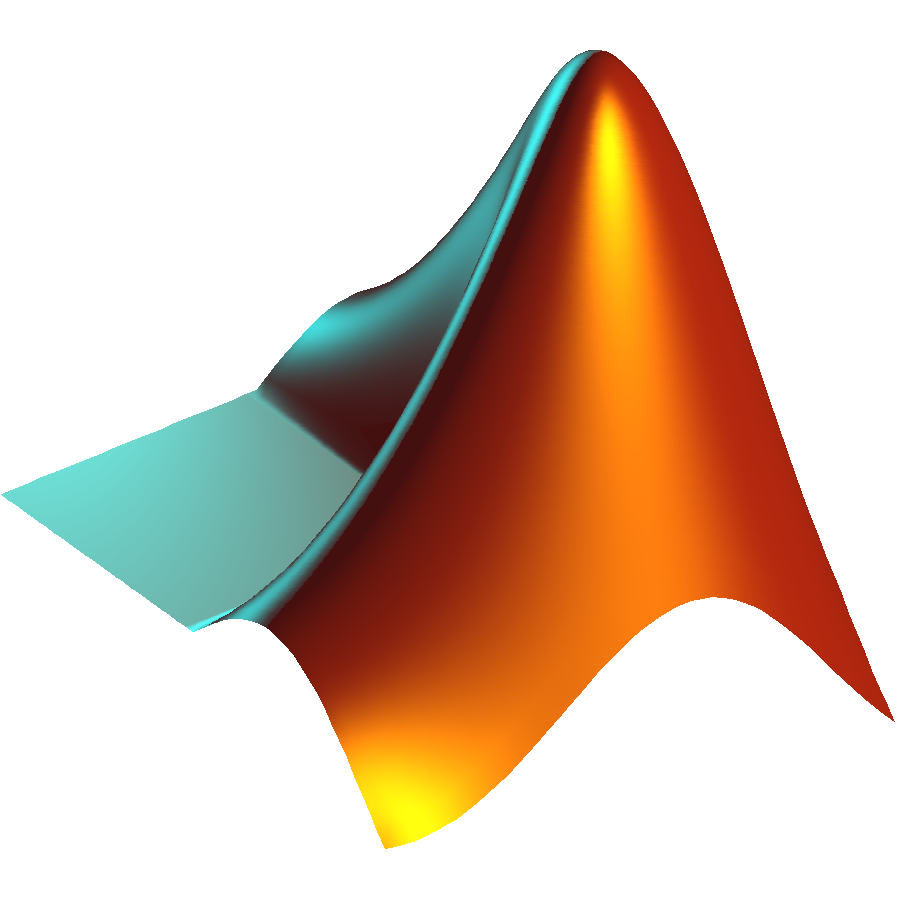
\includegraphics[width=16pt]{matlab-logo.png}};
   \end{tikzpicture}%
  \end{minipage}%
	\begin{minipage}{.8\textwidth}\flushleft
  }
{
\end{minipage}\par\noindent%
\ignorespacesafterend
\vskip12pt} % Tighter line spacing and white space after remark

% Remark with python logo
\newenvironment{premark}{\par\vskip10pt\small % Vertical white space above the remark and smaller font size
\noindent\ignorespaces\begin{minipage}{20pt}   
   \begin{tikzpicture}[overlay]
   \node[anchor=east,draw=c_code_colframe, line width=1pt, rectangle, rounded corners=2pt,fill=c_code_icon_fill,inner sep=2pt,outer sep=0pt, minimum size=20pt] at (-10pt,0pt){
\includegraphics[width=16pt]{python-logo.pdf}};
   \end{tikzpicture}%
  \end{minipage}%
	\begin{minipage}{.8\textwidth}\flushleft
  }
{
\end{minipage}\par\noindent%
\ignorespacesafterend
\vskip12pt} % Tighter line spacing and white space after remark


\newtcolorbox{qbox}[1][]{
	enhanced jigsaw,
  %width=0.5\textwidth,  %% change
  colback=c_qbox_colback,
  colframe=c_qbox_colframe,
  title={
\includegraphics[width=10pt]{interrogation.pdf}},
  boxrule=2pt,
  breakable,
  %left=10pt,right=10pt,top=20pt,bottom=20pt,
  attach boxed title to top left= {xshift=10pt,yshift*=-\tcboxedtitleheight/2},
  boxed title style={boxrule=0pt,size=small,colback=c_qbox_icon_colback,colframe=c_qbox_icon_colframe},
  before=\par\vspace{3mm},
  #1
}

\newtcolorbox{mhelp}[1][]{
	enhanced jigsaw,
  %width=0.5\textwidth,  %% change
  colback=c_code_colback,
  colframe=c_code_colframe,
  coltitle=c_code_title,
  title={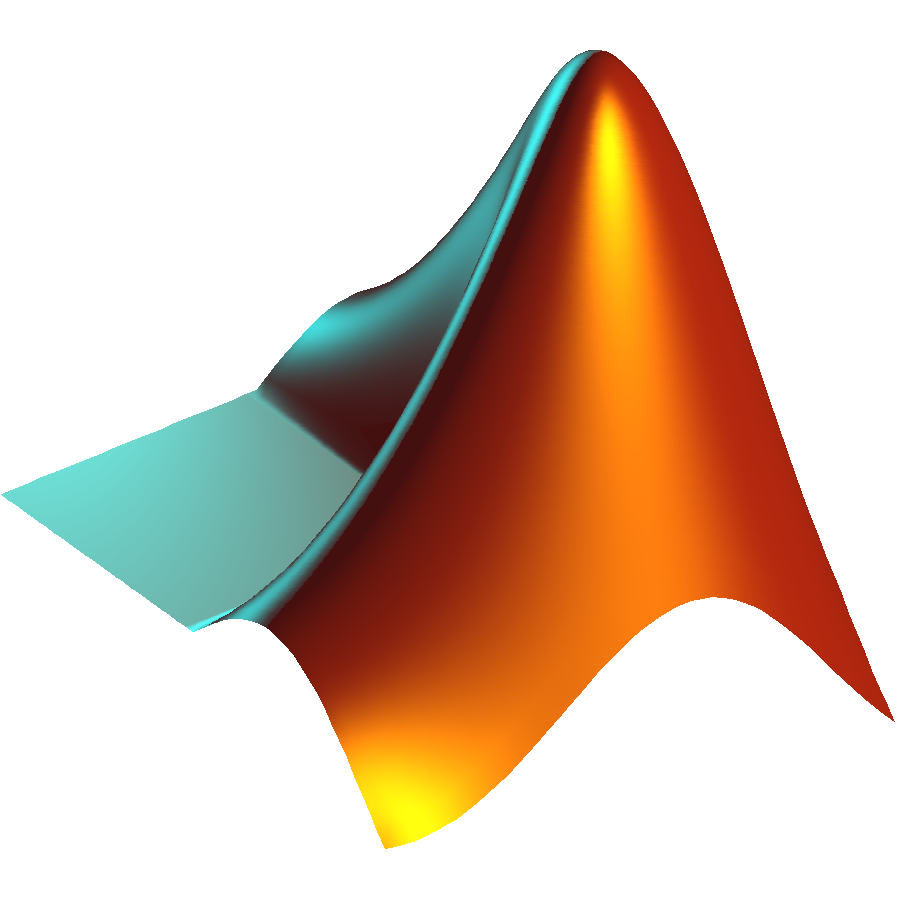
\includegraphics[width=16pt]{matlab-logo.png} Informations},
  boxrule=1pt,
  breakable,
  attach boxed title to top left= {xshift=10pt,yshift*=-\tcboxedtitleheight/2},
  boxed title style={size=small,colback=c_code_colback,colframe=c_code_colframe},
  #1
}


\newtcolorbox{phelp}[1][]{
	enhanced jigsaw,
  %width=0.5\textwidth,  %% change
  colback=c_code_colback,
  colframe=c_code_colframe,
  coltitle=c_code_title,
  title={
\includegraphics[width=16pt]{python-logo.pdf} Informations},
  boxrule=1pt,
  breakable,
  %left=10pt,right=10pt,top=20pt,bottom=20pt,
  attach boxed title to top left= {xshift=10pt,yshift*=-\tcboxedtitleheight/2},
  boxed title style={size=small,colback=c_code_colback,colframe=c_code_colframe},
  #1
}

\usepackage{subfig}

%\usepackage{subcaption}
%\usepackage[table]{xcolor}

% display frame
%\usepackage{showframe}

% maths
\usepackage{amsmath}
\usepackage{amssymb}
\usepackage[cm]{fullpage}
\usepackage[boxed]{algorithm2e}
%\pdfsuppresswarningpagegroup=1

\usepackage{tikz}
\usetikzlibrary{shapes,backgrounds,shapes.misc}
% packages de mise en page
\usepackage[newparttoc]{titlesec} % Allows customization of titles
\usepackage{etoolbox}

%%%%%%%%%%%%%%
% cette partie est due à un bug de texlive
\makeatletter
\patchcmd{\ttlh@hang}{\parindent\z@}{\parindent\z@\leavevmode}{}{}
\patchcmd{\ttlh@hang}{\noindent}{}{}{}
\makeatother

%------------------------------------------------------------------------------
%	MAIN TABLE OF CONTENTS
%------------------------------------------------------------------------------

\usepackage{titletoc} % Required for manipulating the table of contents

\contentsmargin{0cm} % Removes the default margin
% 
% \titleformat{\part}[display]{\center\normalfont\huge\bfseries}
%                             {\partname\ \thepart}{20pt}{\Huge} 

\makeatletter
\renewcommand\contentsname{Table of Contents}
\renewcommand\tableofcontents{%
    \if@twocolumn
      \@restonecoltrue\onecolumn
    \else
      \@restonecolfalse
    \fi
    \chapter*{{\color{c_title}\textsc{\contentsname}}% change here the formatting
        \@mkboth{%
           \MakeUppercase\contentsname}{\MakeUppercase\contentsname}}%
    \@starttoc{toc}%
    \if@restonecol\twocolumn\fi
    }
    \makeatother
    
% titlecontents: style for table of contents
% % % Part text styling
% \titlecontents{part}[1.25cm] % left
% {\addvspace{15pt}\huge\sffamily\bfseries} % above-code
% {\color{c_title}\contentslabel[\huge\thecontentslabel]{1.25cm}\color{c_title}} % numbered-entry-format
% {}  % numberless-entry-format
% {\color{c_title}\huge\titlerule*[1pc]{.}\thecontentspage} % filler-page-format
% [] % below-code
\usepackage{framed}
\renewenvironment{leftbar}
  {\def\FrameCommand{\hspace{6em}%
    {\color{c_title}\vrule width 2pt depth 6pt}\hspace{1em}}%
    \MakeFramed{\parshape 1 0cm \dimexpr\textwidth-6em\relax\FrameRestore}\vskip2pt%
  }
 {\endMakeFramed}
 

\titlecontents{part}
  [0em]{\vspace*{2\baselineskip}}
  {\parbox{4.5em}{%
    \hfill\Huge\sffamily\bfseries\color{c_title}\thecontentspage}%
   \vspace*{-2.3\baselineskip}\leftbar\textsc{\color{c_title}\bfseries\partname~\thecontentslabel}\\\sffamily\bfseries\huge}
  {}{\endleftbar}
  
 %% this is used to put the references as a part in the TOC
\makeatletter
\newcommand{\apppart}[1]{%
  \begingroup
  \patchcmd{\@chapter}
   {\addcontentsline{toc}{chapter}}
   {\addcontentsline{toc}{part}}
   {}{}
  \patchcmd{\@chapter}
   {\addcontentsline{toc}{chapter}}
   {\addcontentsline{toc}{part}}
   {}{}
  \part{#1}
  \endgroup
}
\makeatother
%
% chapter
\titlecontents{chapter}[2.5cm] % Indentation
{\large\sffamily\bfseries} % Spacing and font options for chapters
{\color{c_title}\contentslabel[\Large\thecontentslabel]{.75cm}\color{c_title}} % Chapter number
{} 
{\color{c_rule}\normalsize\sffamily\bfseries\;\titlerule*[.5pc]{.}\;\color{c_title}\thecontentspage} % Page number
[]

% Section text styling
\titlecontents{section}[1.25cm] % Indentation
{\addvspace{5pt}\sffamily\bfseries} % Spacing and font options for sections
{\color{c_title}\contentslabel[\thecontentslabel]{1.25cm}} % Section number
{}
{\color{c_rule}\normalsize\sffamily\bfseries\;\titlerule*[.5pc]{.}\;\color{c_page}\thecontentspage} % Page number
[]

% Subsection text styling
\titlecontents{subsection}[1.25cm] % Indentation
{\addvspace{1pt}\sffamily\small} % Spacing and font options for subsections
{\color{c_section}\contentslabel[\thecontentslabel]{1.25cm}} % Subsection number
{}
{\color{c_page}\sffamily\;\titlerule*[.5pc]{.}\;\thecontentspage} % Page number
[] 
% 
% % subsubsection text styling
% \titlecontents{subsubsection}[1.25cm] % Indentation
% {\addvspace{1pt}\sffamily\small} % Spacing and font options for subsections
% {\color{blueemse!60}\contentslabel[\thecontentslabel]{1.5cm}} % Subsection number
% {}
% {\color{blueemse!60}\sffamily\;\titlerule*[.5pc]{.}\;\thecontentspage} % Page number
% [] 
\usepackage{tcolorbox}

\titleformat{\section}%
	{\normalfont\huge\bfseries\color{c_section}}
	{\llap{\tcbox[colback=c_section_colback, colframe=c_section_colframe, coltext=white, on line, boxsep=0pt, left=4pt, right=4pt, top=4pt, bottom=4pt]{\thesection}}}
	{1em}
	{}

% Section text styling
\titleformat{\subsection}% Indentating
{\Large\sffamily\color{c_section}} % Font settings
{\llap{\thesubsection}}
{0.2em} % sep
{} % before

% Subsection text styling
\titleformat{\subsubsection}% Indentation
{\normalfont\sffamily\color{c_section}} % Font settings
{\thesubsubsection}
{1em}
{}
% 
 % Part text styling
\titleformat{\part}% Indentation
{\Huge\bfseries\color{c_title}} % Font settings
{Part \thepart}
{1em}
{}

%----------------------------------------------------------------------------------------
%	PAGE HEADERS
%----------------------------------------------------------------------------------------
\usepackage[papersize={16.64cm,24.64cm},layoutwidth=16cm, layoutheight=24cm, layouthoffset=0.32cm,layoutvoffset=0.32cm, top=1.5cm,bottom=1.5cm,left=1.7cm,right=1.5cm,headsep=1cm]{geometry} % Page margins
%% format Roman
%\usepackage[papersize={6.25in,9.25in},layoutwidth=6in, layoutheight=9in, layouthoffset=0.125in,layoutvoffset=0.125in, top=1.5cm,bottom=1.5cm,left=1.7cm,right=2cm,headsep=1cm]{geometry} % Page margins
%\usepackage[top=2cm,bottom=2cm,left=2.8cm,right=2.8cm,headsep=1cm]{geometry} % Page margins

\usepackage[]{fancyhdr}
\pagestyle{fancyplain}

\renewcommand{\chaptermark}[1]{\markboth{\sffamily\normalsize\bfseries\color{white} #1}{}} % Chapter text font settings
\renewcommand{\sectionmark}[1]{\markright{\sffamily\normalsize\bfseries\thesection\hspace{5pt}\color{white}#1}{}} % Section text font settings
\fancyhf{} 
%\fancyhead[LE,RO]{\sffamily\normalsize\color{c_section}\thepage} % Font setting for the page number in the header
%\fancyhead[LO]{\color{c_section}\rightmark} % Print the nearest section name on the left side of odd pages
%\fancyhead[RE]{\color{c_section}\leftmark} % Print the current chapter name on the right side of even pages
\renewcommand{\headrulewidth}{0pt} % Width of the rule under the header: 0pt means no rule
\addtolength{\headheight}{2.5pt} % Increase the spacing around the header slightly
\renewcommand{\footrulewidth}{0pt} % Removes the rule in the footer
\fancyhead[LE]{%
  \tikz[remember picture,overlay,baseline]
    \fill[c_qbox_colframe](current page.north west|-0,-\dp\strutbox)
    rectangle(current page.north east);%
  \color{white}\leftmark}
  
\fancyhead[LO]{%
  \tikz[remember picture,overlay,baseline]
    \fill[c_qbox_colframe](current page.north west|-0,-\dp\strutbox)
    rectangle(current page.north east);%
  \color{white}\rightmark}
%\fancyhead[C]{\color{white}Middle part}

\fancyhead[R]{\color{white}\thepage}
\fancypagestyle{plain}{\fancyhead{}\renewcommand{\headrulewidth}{0pt}} % Style for when a plain pagestyle is specified
\usepackage{etoolbox}

\makeatletter
\patchcmd{\@fancyhead}{\rlap}{\color{c_section}\rlap}{}{}
\patchcmd{\headrule}{\hrule}{\color{c_rule}\hrule}{}{}
\patchcmd{\@fancyfoot}{\rlap}{\color{c_section}\rlap}{}{}
\patchcmd{\footrule}{\hrule}{\color{c_rule}\hrule}{}{}
\makeatother

% Removes the header from odd empty pages at the end of chapters
\makeatletter
\renewcommand{\cleardoublepage}{
\clearpage\ifodd\c@page\else
\hbox{}
\vspace*{\fill}
\thispagestyle{empty}
\newpage
\fi}


\usepackage{amsmath,amsfonts,amssymb,amsthm} % For including math equations, theorems, symbols, etc

\def\QRCODE{qrcode}
\def\QRPAGE{qrpage}

\def\difficulty{0}
\def\@makechapterhead#1{
\thispagestyle{empty}
{\centering \normalfont\sffamily
\ifnum \c@secnumdepth >\m@ne
\if@mainmatter
\startcontents
\begin{tikzpicture}[remember picture, overlay]
\node at (current page.north west)
{
\begin{tikzpicture}[remember picture,overlay]

\node (dummy)[anchor=north west]  at (-2cm, -2.5cm){}; % pour faire continuer le cadre a l'exterieur
\node (number)[anchor=north west] at (2cm, -2.5cm) {\huge\sffamily\bfseries\textcolor{c_section} {\thechapter}};
\ifthenelse{\difficulty>0}{
\foreach \i in {1,...,\difficulty}{
  \node [star,fill=c_title,anchor=north east,scale=0.5] at (2cm - 0.3*\i cm, -2.5cm) {};
  }
}{TEST}
\node (section) [anchor=north west, text width=\textwidth-1.5cm] at (3.5cm, -2.5cm) {\huge\sffamily\bfseries\textcolor{c_section} {#1}};%\vphantom{plPQq}
 \node (exterieur) [anchor=west,rounded corners=25pt,draw=c_section,draw opacity=1,line width=2pt,inner sep=12pt,fit={(dummy) (number) (section)}] {};

\end{tikzpicture}};
\end{tikzpicture}}\par\vspace*{2cm}
\fi
\fi
}

\newcommand{\genericcorrectionsection}[2]{%
\vspace{1cm}
\noindent\begin{tikzpicture}[remember picture,overlay]
\node (dummy)[anchor=text]  at (-5cm, 0cm){}; % pour faire continuer le cadre a l'exterieur
\node (section) [anchor=text] {\Large\sffamily\bfseries\textcolor{c_section} {\stepcounter{section}\thesection. #1}};
\node (qr) [right=of section,anchor=west] {\href{\QRPAGE}{\includegraphics[height=1.5cm]{\QRCODE}}};
\node (logo) [anchor=text] at (-1.5cm, -0.1cm) {\includegraphics[height=1cm]{#2}};
\begin{scope}[on background layer]\node (exterieur) [anchor=text,rounded corners=10pt,fill=c_section_colback, draw=c_section_colframe,draw opacity=1,line width=2pt,inner sep=4pt,fit={(dummy) (section) (qr)}] {};
\end{scope}

\end{tikzpicture}
\phantom{#1}
\vspace{.6cm}
%\noindent\makebox[\linewidth]{\color{orange}\rule{\textwidth}{2pt}} 
}

\newcommand{\correctionsection}[1]{%
\genericcorrectionsection{#1}{interrogation.pdf}
}
\newcommand{\mcorrectionsection}[1]{%
\genericcorrectionsection{#1}{matlab-logo.png}
}
\newcommand{\pcorrectionsection}[1]{%
\genericcorrectionsection{#1}{python-logo.pdf}
}



\setcounter{tocdepth}{0}


%%%%%%%%%%%%%%%%%%%%%%%%%%%%%%%%%%%%%%%%%%%%%%%%%%%%
%% NOUVEAUX ENVIRONNEMENTS %%
%% DONNEES PREAMBULE %%
\def\Dannee{~}
\def\Dmodule{~}
\def\Dmatiere{~}
\def\Dtype{~}
\newcommand{\annee}[1]{\def\Dannee{#1}}
\newcommand{\module}[1]{\def\Dmodule{#1}}
\newcommand{\matiere}[1]{\def\Dmatiere{#1}}
\newcommand{\type}[1]{\def\Dtype{#1}}

\makeatletter
\def\sujet{\@ifnextchar[{\@sujetwith}{\@sujetwithout}}
\def\@sujetwith[#1]#2{\chapter[#1]{#2}}
\def\@sujetwithout#1{\chapter{#1}}
\makeatother
%\newcommand{\sujet}[2]{\ifthenelse{\equal{#2}{}}{\chapter{#1}}{\chapter[#2]{#1}}}
%{\vspace*{0.0cm}\begin{center}{\LARGE{\bfseries \Dtype : #1}}\end{center}\vspace{0.75cm}}

\tikzstyle{mybox} = [draw=c_section_colframe, fill=c_section_colback, very thick,
    rectangle, rounded corners, inner sep=10pt, inner ysep=20pt]
\tikzstyle{fancytitle} =[fill=c_section_colframe, text=white]

% \newcommand{\note}[1]
% {\begin{tikzpicture}%
% \node [mybox, text width=.9\textwidth, align=justify] (box){%
%   %  \begin{minipage}{.95\textwidth}%
%      \color{c_section}{#1} %
%   %  \end{minipage}%
%     };%
% \node[fancytitle, right=10pt] at (box.north west) {Note};%
% \end{tikzpicture}%
% \vspace*{0.5cm}}


\newtcolorbox{note}[1][]{%
  colback=c_section_colback,colframe=c_section_colframe,
  #1}

\newtcolorbox{rmq}[1][]{%
  colback=lightgray,colframe=black,
  #1}


\newcounter{exonumber}[chapter]
\newenvironment{exo}[1]
{\par\stepcounter{exonumber}\noindent
{\pagebreak[1]\\
\rule[0ex]{\textwidth}{0.1mm}\\
\noindent\bf\uppercase{Exercice} \theexonumber.}\quad{\bfseries\itshape
  #1\\
\rule[2ex]{\textwidth}{0.1mm}}\noindent
\begin{samepage}}
{\end{samepage}}

\newcounter{questionnumber}
\newenvironment{question}[1]
{\par\stepcounter{questionnumber}\noindent
{\bf\uppercase{Question} \thequestionnumber.}\quad{\bfseries\itshape #1}\par\begin{maliste}}
{\end{maliste}\bigskip}

\newenvironment{maliste}%
{ \begin{list}%
	{$\square$}%
	{}}%
{ \end{list} }
%%%%%%%%%%%%%%%%%%%%%%%%%%%%%%%%

\newcommand{\N}{\mathbb{N}}
\newcommand{\R}{\mathbb{R}}
\DeclareMathOperator*{\argmin}{arg\,min}
\DeclareMathOperator*{\divergence}{div}
\DeclareMathOperator*{\grad}{grad}

\newcount\colveccount
\newcommand*\colvec[1]{
        \global\colveccount#1
        \begin{pmatrix}
        \colvecnext
}
\def\colvecnext#1{
        #1
        \global\advance\colveccount-1
        \ifnum\colveccount>0
                \\
                \expandafter\colvecnext
        \else
                \end{pmatrix}
        \fi
}

% ensembles mathématiques
\def\E{{\mathbb{E}}}
\def\fft{{\mathcal{F}}}

\usepackage{pdf14}
\pdfminorversion=4
\setlength{\headheight}{15pt}
\usepackage{makeidx}
% commandes communes entre book et tutorials

\makeatletter
% commande utilisée pour faire une référence croisée entre tutoriels
\newcommand{\iflabelexists}[3]{\@ifundefined{r@#1}{#3}{#2}}
\makeatother
\usepackage{placeins}

\usepackage{pgfplots}
  \pgfplotsset{compat=newest}
  %% the following commands are sometimes needed
  \usetikzlibrary{plotmarks}
  \usepackage{grffile}
  \usepackage{amsmath}
  
 % package pour l'insertion d'un espace intelligent
\usepackage{xspace}
% tilde in math mode
\renewcommand{\t}[1]{\ensuremath{\mathop{\tilde{#1}}\nolimits}}
\newcommand{\h}[1]{\ensuremath{\mathop{\hat{#1}}\nolimits}}
\newcommand{\lab}{$L^*a^*b^*$\xspace}
\newcommand{\argyb}{$(a,rg,yb)$\xspace}
\newcommand{\targyb}{$(\tilde{a},\tilde{rg},\tilde{yb})$\xspace} % tilde
\newcommand{\cargyb}{$(\h{a},\h{rg},\h{yb})$\xspace} % espace chapeau
% TIKZ and diagrams
\usepackage{pgf,tikz}
\usetikzlibrary{arrows,shapes,matrix,positioning}
% styles de block pour diagrammes
\tikzset{decision/.style={diamond, draw, fill=blue!20, text width=1.5cm, text badly centered, inner sep=0pt, minimum width=3.5cm}}
\tikzset{block/.style={rectangle, draw, fill=blue!20, text width=3cm, text badly centered, rounded corners,
minimum width=3cm}}
\tikzset{dligne/.style={draw, latex-latex}}
\tikzset{ligne/.style={draw, -latex}}

\tikzset{title/.style={font=\fontsize{6}{6}\color{black!50}\ttfamily}}
\tikzset{typetag/.style={rectangle, draw=black!50, font=\scriptsize\ttfamily, anchor=west}}


